\documentclass[../main.tex]{subfiles}

\begin{document}



Mạng nơ-ron hồi quy là một lớp trong các mạng nơ-ron nhân tạo. Với các mạng nơ-ron thông truyền, có một giả thuyết được đặt ra là tất cả các đầu vào và đầu ra là độc lập với nhau. Tuy nhiên điều này lại không đúng với rất nhiều những bài toán. Ví dụ để dự đoán một từ ở trong câu, việc nhận biết, nắm bắt thông tin của các từ trước đó là cần thiết. Khi đó mạng nơ-ron hồi quy sẽ hoạt động theo cơ chế trên. Theo nghiên cứu \cite{liu2014recursive}, lý do chính để sử dụng mạng nơ-ron hồi quy là để xử lý thông tin dạng chuỗi. Và phần "hồi quy" trong mạng chính là kết quả khi thực hiện cùng một biến đổi cho mọi phần tử của chuỗi đầu vào và đầu ra phụ thuộc vào các tính toán trước đó. Về lý thuyết, cách mà mạng nơ-ron hồi quy có thể biểu diễn như thể mạng này có bộ nhớ để lưu trữ lịch sử về các phần tử đã xử lý trước đó. Vì thế tại mỗi thời điểm, các tính toán trước đó đều được sử dụng để dự đoán đầu ra tiếp theo từ quá trình. 

\begin{figure}[t]
\centering
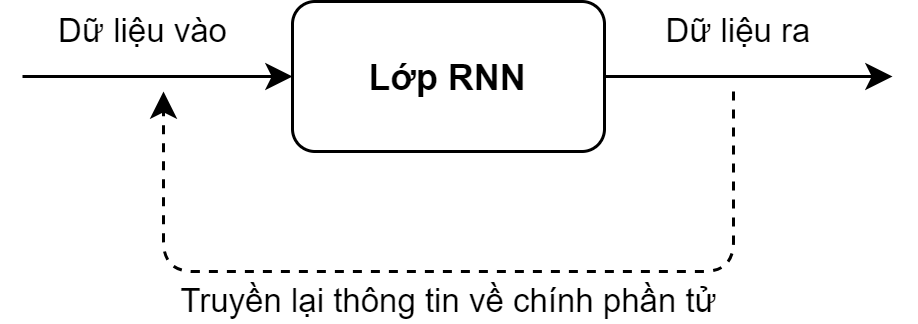
\includegraphics[scale=0.4]{02-RNN}
\caption{Mô hình mạng nơ-ron hồi quy}
\end{figure}

\begin{figure}[t]
\centering
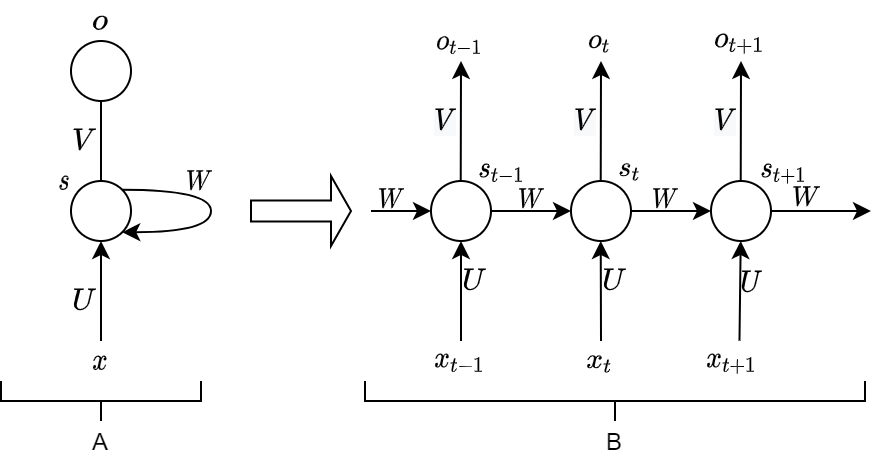
\includegraphics[scale=0.4]{02-unfold-RNN}
\caption{Mô hình mạng nơ-ron hồi quy chưa phân rã và đã phân rã}
\end{figure}

Trong hình $2.4$ có mục A mô tả trạng thái chưa phân rã của mạng nơ-ron hồi quy và hình B mô tả mạng nơ-ron hồi quy khi phân rã thành các mạng con. Từ mục B có thể quan sát rằng giả sử có $3$ tầng mạng nơ-ron. Trong hình cũng có đề cập đến $3$ tham số $U$, $V$, $W$ dùng cho việc tính toán mạng RNN. Đó là $3$ tham số biểu diễn trọng số của các nơ-ron. Ví dụ, $W$ biểu diễn trọng số của các nốt nằm trong trạng thái ẩn $S$. $V$ biểu diễn trọng số của các nốt giữa các trạng thái ẩn $S$ và đầu ra $O$. $U$ biểu diễn trọng số của các nốt giữa đầu vào X và trạng thái ẩn $s$. Điểm khác biệt giữa RNN và mạng nơ-ron truyền thống là $3$ tham số này không luôn có cùng một giá trị, nhưng trong mạng nơ-ron truyền thống thì đây là các tham số thay đổi. Có được điều này là bởi vì cùng một nhiệm vụ sẽ được thực hiện với mỗi tham số đầu vào. 

- $x_{t}$ là đầu vào tại thời gian $t$. Ví dụ $x_0$ là một vector one-hot tương ứng với từ đầu tiên của một câu. 

- $s_{t}$ là trạng thái ẩn tại thời gian $t$. Đây chính là bộ nhớ của mạng. $s_{t}$ được tính dựa vào trạng thái ẩn trước đó $s_{t-1}$ và đầu vào tại trạng thái hiện tại.

- $s_{t} = f(Ux_{t} + Ws_{t-1})$

Hàm $f$ thường là hàm phi tuyển tính như $tanh$ hoặc $ReLU$. $s_{0}$ được gán là $0$. 

- $o_{t}$ là đầu ra tại thời gian t. $o_{t} = softmax(Vs_{t})$

Khi huấn luyện mô hình sẽ sử dụng chung tham số về các nốt tại mọi thời điểm, vì thế đạo hàm tại mỗi đầu ra phụ thuộc vào các bước tính toán hiện tại và trước đó. Ví dụ, để tính đạo hàm tại $t = 4$, mô hình sẽ phải truyền ngược về $t = 3$ và lấy tổng các đạo hàm trước đó. Quá trình này gọi là truyền ngược theo thời gian (Back Propagatiton Through Time - BPTT).

Tuy nhiên xuất hiện những người hợp mô hình cần nhiều ngữ cảnh hơn để đưa ra được đầu ra hợp lý. Điều này đặt ra vấn đề về phụ thuộc xa. Về lý thuyết, mạng nơ-ron hồi quy hoàn toàn có thể xử lý vấn đề này. Với sự can thiệp của con người để chọn ra tham số thích hợp thì vấn đề có thể được giải quyết. Thế nhưng trong thực tiễn, mô hình RNN không cho thấy khả năng đó. Điều này được chỉ ra bởi\cite{bengio1994learning}


\end{document}